\subsection{Definitions}
\label{mls:definitions}

There are multiple definitions within Chapter \ref{chap:prediction_based_scheduler} that will be used as a part of the multi-level security extension. There will also be changes to existing definitions and new definitions to properly implement and define the prediction-based solution within multi-level secure databases.

Definitions \ref{mls:cmt_rate} \& \ref{mls:eff_rate} are references of Definitions \ref{cmt_rate} \& \ref{eff_rate} from Chapter \ref{chap:prediction_based_scheduler}. Both of which will remain unchanged and will provide a base for the three-dimensional model presented in this model.

\begin{definition}
\label{mls:security_classification}
(Security Classification) - the security classification of a transaction $T_{i}$, denoted as  $S_{c}(T_{i})$, is based on the level of access assigned to the transaction based either on the information it's accessing or the authenticated user initiating the transaction. The security classification by resource is calculated as follows:

\begin{center}
Let $R_{all} = \{R_1, R_2,... R_n\}$ be the set of all resources accessed by transaction $T_i$. \newline
Then $S_c(T_i)$ is denoted by the max security classification of $R_{all}$.

$S_c(T_i) = S_c(MAX(R_{all}))$
\end{center}

The security classification calculated by user is calculated as follows:

\begin{center}
Let $S_C(U_{bob})$ be the security classification of user Bob.\newline 
If $T_i$ is initiated by $U_{bob}$ then $S_C(T_i) = S_C(U_{bob})$
\end{center}

\end{definition}

\defCommitRate{mls:cmt_rate}
\defEfficiencyRate{mls:eff_rate}

Definition \ref{transaction_categories} in Chapter \ref{chap:prediction_based_scheduler} established a four category system that was the basis of the prediction-based categorization solution. This solution must be extended within multi-level secure databases in order to account for the security levels. Definition \ref{mls:transaction_categories} extends this categorization to eight categories to account for high and low security classifications. The additional categorizations also allow for the three dimensional categorization structure.

\begin{definition}
\label{mls:transaction_categories}
(MLS Transaction Categories) - Let $T$ = \{$T_{1}$, ... , $T_{n}$\} be a set of transactions and $C$ = \{$HCHE_H$, $HCLE_H$, $LCHE_H$, $LCLE_H$, $HCHE_L$, $HCLE_L$, $LCHE_L$, $LCLE_L$\} a set of category names. The mapping $\tau$ associates a category name with each transaction as follows:

\[ 
\tau : \textrm{$T_{i}$}\rightarrow
\left \{
  \begin{tabular}{cc}
  $HCHE_H$ & if $C_{r}(T_{i}) > 0.5$ and $E_{r}(T_{i}) > 1$ and $S_{level}$ = $HIGH$ \\
  $HCLE_H$ & if $C_{r}(T_{i}) > 0.5$ and $E_{r}(T_{i}) \le 0.5$ and $S_{level}$ = $HIGH$ \\
  $LCHE_H$ & if $C_{r}(T_{i}) \le 0.5$ and $E_{r}(T_{i}) > 1$ and $S_{level}$ = $HIGH$ \\
  $LCLE_H$ & if $C_{r}(T_{i}) \le 0.5$ and $E_{r}(T_{i}) \le 0.5$ and $S_{level}$ = $HIGH$ \\
  $HCHE_L$ & if $C_{r}(T_{i}) > 0.5$ and $E_{r}(T_{i}) > 1$ and $S_{level}$ = $LOW$ 
  \\
  $HCLE_L$ & if $C_{r}(T_{i}) > 0.5$ and $E_{r}(T_{i}) \le 0.5$ and $S_{level}$ = $LOW$ \\
  $LCHE_L$ & if $C_{r}(T_{i}) \le 0.5$ and $E_{r}(T_{i}) > 1$ and $S_{level}$ = $LOW$ \\
  $LCLE_L$ & if $C_{r}(T_{i}) \le 0.5$ and $E_{r}(T_{i}) \le 0.5$ and $S_{level}$ = $LOW$
  \end{tabular}
\right \}
\]

{\normalfont The addition of a third categorization attribute (security classification level) introduces four additional categories and a third dimension on top of the existing model presented in Definition \ref{transaction_categories} in Chapter \ref{chap:prediction_based_scheduler}.
}

\end{definition}




\begin{definition}
\label{mls:cat_dominance}
(MLS Transaction Category Dominance) - The Transaction Category Dominance is a pair, denoted as $C_{D} = (C,L)$, where $C$ is the set of transaction categories, and $L$ is a partial order of the categories such that:
 
\[\textrm{$HCHE_L > HCLE_L > LCLE_L > HCHE_H > HCLE_H > LCLE_H$}\]
\[\textrm{$HCHE_L > LCHE_L > LCLE_L > HCHE_H > LCHE_H > LCLE_H$} \]

\begin{figure}[h]
\captionsetup{justification=centering}
\centering % used for centering Figure

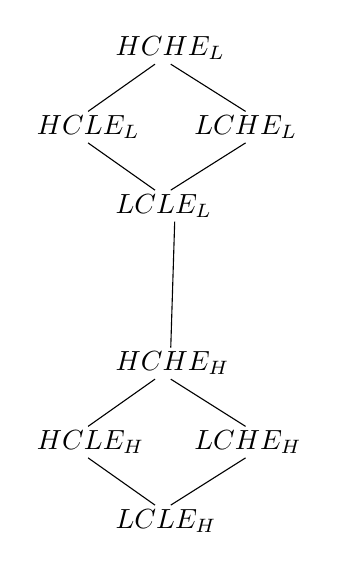
\begin{tikzpicture}
    % [list/.style={rectangle split, rectangle split parts=3,
    % draw, rectangle split horizontal}, >=stealth, start chain]
  \node[text width=1.5cm] at (3.8,5) {$HCHE_H$};
  \node[text width=1.5cm] at (2.8,4) {$HCLE_H$};
  \node[text width=1.5cm] at (4.8,4) {$LCHE_H$};
  \node[text width=1.5cm] at (3.8,3) {$LCLE_H$};
  \node[text width=1.5cm] at (3.8,9) {$HCHE_L$};
  \node[text width=1.5cm] at (2.8,8) {$HCLE_L$};
  \node[text width=1.5cm] at (4.8,8) {$LCHE_L$};
  \node[text width=1.5cm] at (3.8,7) {$LCLE_L$};
  \draw (3.55,4.8) -- (2.7,4.2);
  \draw (3.75,4.8) -- (4.7,4.2);
  \draw (3.55,3.2) -- (2.7,3.8);
  \draw (3.75,3.2) -- (4.7,3.8);
  \draw (3.55,8.8) -- (2.7,8.2);
  \draw (3.75,8.8) -- (4.7,8.2);
  \draw (3.55,7.2) -- (2.7,7.8);
  \draw (3.75,7.2) -- (4.7,7.8);
  \draw (3.8,6.8) -- (3.75,5.2);
  
\end{tikzpicture}

% \caption{Web Service Environment with Scheduler} % title of the Figure
\label{fig:mls_category_lattice} % label to refer figure in text

\end{figure}

{\normalfont Note that the categories $HCLE$ and $LCHE$ (in both security classifications) are not comparable. That is, we cannot establish a dominance relation between transactions in $HCLE$ and $LCHE$ categories.

However, in our security model, we focus on removing the timing covert security channel. Therefore, we prioritize the efficiency property over the commit property. We introduce the dominance relation below in Table \ref{tbl:mls_priority}.}

\[\textrm{$LCHE > HCLE$} \]
 
\begin{table}[h]
\captionsetup{justification=centering}
\centering
\begin{tabular}{l|c|}
\cline{2-2}
                                          & \multicolumn{1}{l|}{\textbf{Priority}} \\ \hline
\multicolumn{1}{|l|}{\textbf{HCHE}}  & I                                      \\ \hline
\multicolumn{1}{|l|}{\textbf{LCHE}}  & II                                     \\ \hline
\multicolumn{1}{|l|}{\textbf{HCLE}} & III                                     \\ \hline
\multicolumn{1}{|l|}{\textbf{LCLE}} & IV                                      \\ \hline
\end{tabular}

\caption{MLS Category Priorities} % title of the Figure
\label{tbl:mls_priority} % label to refer figure in text

\end{table} 
\end{definition}

Definition \ref{mls:conflict_ops} is adapted from Definition \ref{conflict_ops} in Chapter \ref{chap:prediction_based_scheduler}. Here we add the distinctions needed to adapt the existing model to MLS databases.

\begin{definition}
\label{mls:conflict_ops}
 (MLS Conflicting Operations) - two operations are conflicting:

 \begin{enumerate}
   \item they are contained within two different transactions,
   \item both operations are operating on the same data item
   \item at least one of the operations is a WRITE, and
   \item the security classifications differ
 \end{enumerate}

 \begin{example}
 \label{mls:ex_conflict_ops}
  Let $o_{1}$ be a READ operation on data item $r_{a}$ in transaction $T_{1}$ and let $o_{2}$ be a WRITE operation on $r_{a}$ in $T_{2}$. Let $S_C(T_1) <> S_C(T_2)$. These two operations are conflicting.
 \end{example}
\end{definition}